\documentclass[class=minimal,border=1cm]{standalone}
\usepackage{tikz}
%\usepackage{fullpage}

\newcommand\LW{2}
\newcommand\CMB{0}
\begin{document}

%\section*{Wiring diagram}
%\section{Licence}
%BBC:Micro:bit image from the microbit Educational Foundation at microbit.org (https://github.com/microbit-foundation/microbit-svg.git)

\begin{tikzpicture}

\node (top) at (0,5) {Vorname:\hspace{15em} Team:\hspace{15em} Roboter:\hspace{10em},};

%\node[rotate=90] (motordriver) at (0,1)
\node[rotate=90] (motordriver) at (-5,2)
{
%\includegraphics[width=0.9\textwidth]{fig/MotorDriverV2}
};
%\node (microbit) at (0,5.5)
\node (microbit) at (\CMB,1)
{
\def\svgwidth{0.4\columnwidth}
\input{fig/microbit-svg/microbit-drawing.pdf_tex}
};

% pin 0, 1, 2
\draw[line width=1em, color=black!30] (\CMB-2.50,-1.3) -- (\CMB-2.50,-\LW);
\draw[line width=1em, color=black!30] (\CMB-1.30,-1.3) -- (\CMB-1.30,-\LW);
\draw[line width=1em, color=black!30] (\CMB+0.03,-1.3) -- (\CMB+0.03,-\LW);
% +3V
\draw[line width=1em, color=red!70] (\CMB+1.37,-1.3) -- (\CMB+1.37,-\LW);
% GND
\draw[line width=1em, color=black!70] (\CMB+2.55,-1.3) -- (\CMB+2.55,-\LW);

% Motors
%\node[rotate=-89] (m1) at (-6.5,-4){ 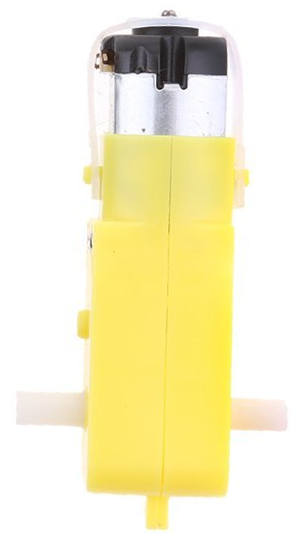
\includegraphics[scale=0.25]{fig/DCMotor-crop} };
%\node[rotate=-89] (m2) at (-6.5,-7){ 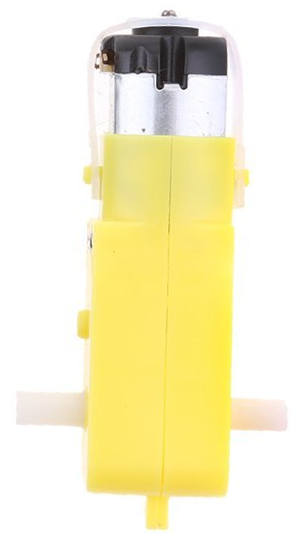
\includegraphics[scale=0.25]{fig/DCMotor-crop} };
\node[] (bb) at (0,-12) {\includegraphics[width=0.25\textwidth]{fig/Breadboard2}};

% Empty slots left
%\draw (-9,-2) rectangle (-4,-5);
\draw (-9,-5.5) rectangle (-4,-8.5);
\draw (-9,-9) rectangle (-4,-12);
\draw (-9,-12.5) rectangle (-4,-15.5);
\draw (-9,-16) rectangle (-4,-19);

% Empty slots right
%\draw (4,-2) rectangle (9,-5);
\draw (4,-5.5) rectangle (9,-8.5);
\draw (4,-9) rectangle (9,-12);
\draw (4,-12.5) rectangle (9,-15.5);
\draw (4,-16) rectangle (9,-19);

\end{tikzpicture}

\end{document}
